\documentclass[a4paper,11pt]{article}
\usepackage[top = 1.5 in, bottom = 1 in, left = 1 in, right = 1 in]{geometry}
\usepackage[utf8]{inputenc}
\usepackage[T1]{fontenc}
\usepackage{csquotes}
\usepackage[british]{babel}
\usepackage{lmodern}
\usepackage{url}
\usepackage{color}
\usepackage{graphicx}
\usepackage{setspace}
\usepackage{pdfpages}

\begin{document}
\title{Course project: Mini-PL interpreter}
\author{Laura Leppänen \\ Student number: 013302782 \\ Compilers, Spring 2012}
\date{\today}
\maketitle
\thispagestyle{empty}

\tableofcontents
\onehalfspacing

\newpage
\setcounter{page}{1}

\section{Interpreter implementation}

This section covers the general architecture of the interpreter, testing, building and running instuctions etc.

\subsection{Architecture}

\begin{figure}
    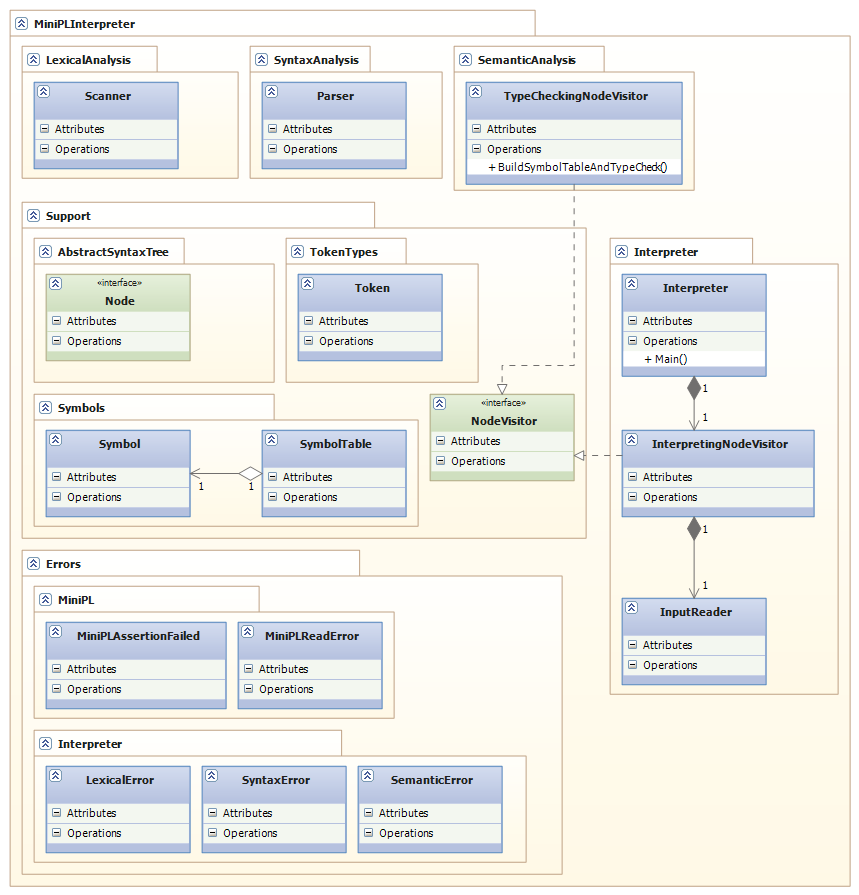
\includegraphics[scale=0.7]{architecture.png}
    \caption{The architecture of the interpreter (exluding different token and node classes and package imports to maintain clarity).}
\end{figure}

\subsection{Error handling}

\subsection{Testing}

\subsection{Building and running the interpreter}

\section{The Mini-PL language}

This section covers issues related to scanning and parsing Mini-PL: token patterns, the context-free grammar, and the abstract syntax tree.

\subsection{Mini-PL token patterns}

\begin{table}[h!]
\begin{tabular}{| l | l |}
    \hline
    Token type & Regular expression \\
    \hline
    Variable or keyword \textsuperscript{1} & [a-zA-Z][0-9a-zA-Z]* \\
    \hline
    Integer literal & [0-9][0-9]* \\
    \hline
    String literal \textsuperscript{2} & "([\^{}"\textbackslash]|(\textbackslash[\textbackslash tnrv"]))*" \\
    \hline
    Endline symbol & ; \\
    \hline
    Assignment symbol & := \\
    \hline
    Colon symbol (type declaration) & : \\
    \hline
    Operator symbols \textsuperscript{3} & +|-|*|<|/|=|\&|! \\
    \hline
    Parentheses & (|) \\
    \hline
    Range operator & .. \\
    \hline
\end{tabular}
\end{table}

Notes:
\begin{enumerate}
\item Matching patterns are identified as keywords or variables by checking a predefined keyword list.
\item String literals can contain any characters except non-escaped quotes or backslashes. Valid escape characters are \verb \\ , \verb \n , \verb \t , \verb \v , \verb \r , \verb \" . Note that backslash characters in the regex are character literals with no special escape meaning.
\item The specification lists \verb,!, as a binary operator as well as a unary operator. Because the specification did not specify the meaning of \verb,!, as a binary operator, I assumed it was mistakenly listed as such and only accepted it as a unary operator. The division operator symbol / is special because it can also begin a comment.
\end{enumerate}

Non-token patterns:
\begin{table}[h!]
\begin{tabular}{| l | l |}
    \hline
    Whitespace & (\textbackslash t|\textbackslash r|\textbackslash n|\textbackslash v| )* \\
    \hline
    Single line comment & //[\^{}\textbackslash n]*\textbackslash n \\
    \hline
    Multiline comment (\textbackslash * is an asterisk symbol) & /\textbackslash *.*\textbackslash */ \\
    \hline
\end{tabular}
\end{table}

\subsection{Context-free grammar}

Refer to appendices for the original non-LL(1) grammar. I have renamed \verb,<stmts>, to \verb,<stmt-list>,. \verb,\epsilon, denotes the empty string.

\begin{verbatim}
<prog>           ::= <stmt-list>
<stmt-list>      ::= <stmt> ";" <stmt-list-tail>
<stmt-list-tail> ::= <stmt-list>
                  | \epsilon
<stmt>           ::= "var" <var-ident> ":" <type> <opt-assignment>
                  |  <var-ident> ":=" <expr>
                  |  "for" <var_ident> "in" <expr> ".." <expr>
                     "do" <stmt-list> "end" "for"
                  |  "read" <var-ident>
                  |  "print" <expr>
                  |  "assert" "(" <expr> ")"
<opt-assignment> ::= ":=" <expr>
                  |  \epsilon
<expr>           ::= <opnd> <expr-tail>
                  |  <unary-op> <opnd>
<expr-tail>      ::= <op> <opnd>
                  |  \epsilon
<opnd>           ::= <int>
                  |  <string>
                  |  <var-ident>
                  |  "(" <expr> ")"
<type>           ::= "int" | "string" | "bool"
<var-ident>      ::= <ident>
\end{verbatim}

\subsection{Abstract syntax trees}

\appendix
\section{Appendices}

Starting on the next page.

\includepdf[pages={1, 2}]{project_spec.pdf}

\includepdf[pages={1, 2}]{minipl_spec.pdf}

\end{document}
